\documentclass[a4paper,twoside,11pt]{book}
\usepackage{a4wide,amsmath,amssymb,verbatim}%,oz}
\usepackage{listings,amsthm}
\usepackage[pdftex]{color,graphicx}
\usepackage[pdftex,colorlinks]{hyperref}
\usepackage{subfig}
\lstset{language=Pascal,basicstyle=\small}

\setlength{\parindent}{0pt}
\setlength{\parskip}{2ex}

\theoremstyle{plain} \newtheorem{powerup}{Power-Up}

\begin{document}

   \begin{titlepage}
        {\ }\\[5.0cm]
        { {\Large OGO 3.1 spring 2009}}\\[0.2cm]
        {\bf \Huge Bomb3D Manual}\\[0.1cm]
        { {\Large {Computer Science, TU/e} }}\\[1.0cm]
        {\ Eindhoven, \today }\\[0.2cm]
		  {\ $ $Rev: 225 $ $ }\\[0.2cm]
        \begin{flushright}
            {\bf {\small Group 2 }}\\[0.0cm]
            {\em {\small Etienne van Delden, 0618959}}\\
            {\em {\small Edin Dudojevic, 0608206}}\\
            {\em {\small Jeroen Habraken, 0586866}}\\
            {\em {\small Neal van den Eertwegh, 0610024 }}\\
            {\em {\small Stef Louwers, 0590864}}\\
            {\em {\small Leroy Bakker, 0617167}}\\
            {\em {\small Anson van Rooij, 0596312}}\\[0.5cm]
        \end{flushright}
    \end{titlepage}
    \tableofcontents



\chapter{Introduction} % (fold)
\label{cha:introduction}

\section{The creators bid you welcome!} % (fold)
\label{sec:the_creators_bid_you_welcome_}

Hi, and thanks for purchasing, pirating or otherwise acquiring Bomb3D! You've made a first step on the road to fame, fortune, death and endless hours of fun blasting away your friends in a virtual, and quite hazardous, 3D environment!

% section the_creators_bid_you_welcome_ (end)

\section{The story} % (fold)
  \label{sub:the_story}

   The year is 2176 and the darkest predictions about our future have come true. Humankind has grown far beyond the ability to sustain itself with earth's limited resources, and shortages are everywhere. Robots have taken over most jobs, virtual realities prevent the rich from facing the problems of the poor, and many biotechnology nightmares have come true. In this dystopian world, most of the earth's population lives in sprawling, metropolitan cities with ineffective, corrupt law enforcement, which have come under the control of all kinds of criminal organisations. The poor jobless masses have few career options, most of them illegal, and drug trafficking, muggings and violent gang wars are only a few of their problems. Because of this, the prison population has exploded, and people are desperate and unruly. The governments' solution is entertainment. Cruel entertainment. \\

    All over the world, tournaments are held, in which prisoners are pitted against insane thrill seekers, professional gladiators, and unfortunates with powerful enemies, to serve as entertainment for the repressed masses. In these tournaments, men and women fight each other with various types of dangerous bombs and weapons provided by their patrons, plus whatever is to be found in the arena. They must use the lay-out of the battlefield and the weapons available in ever more clever ways to have a shot at freedom, fame and fortune. The object of the tournaments is simple: \\

\begin{center}
\textbf{It is to kill \ldots or be killed}    
\end{center}


% chapter introduction (end)

\chapter{Installation} % (fold)
\label{cha:installation}

    \section{System Requirements} % (fold)
    \label{sec:system_requirements}
        During the writing of this document, we have not yet established the exact requirements. We do have the following information.
        
        \begin{tabular}{l|l}
            Operating System & Linux, Windows XP/7 and Mac OS X 10.5 ``Leopard'' \\
                                 & (Others systems have not been tested )\\
            CPU              & Intel Processor \\
            Harddisk         & 100 mb free space \\
            Software         & A working python 2.5.x/2.6.x install, with PyOpenGL and Pygame\\
            Network          & Wireless or wired network (users must be in the same subnet) 
        \end{tabular}
        
        
    % section system_requirements (end)

    \section{Installing the game} % (fold)
    \label{sec:installing_the_game}
        Before you can play this fantastic game, you must install it. We currently don't have an installer, so Python and the PyOpenGL and PyGame python modules are required to play this game. To install the game, just extract the archive to the desired installation directory.
    % section installing_the_game (end)

    \section{Starting the Game} % (fold)
    \label{sec:starting_the_game}
        To start the game, open up a terminal (Linux, Mac OS X) or command prompt (windows) and change into the directory that has the Bomb3d installation (Figure~\ref{fig:directory}).
        
        \begin{figure}[!ht]
          \centering
          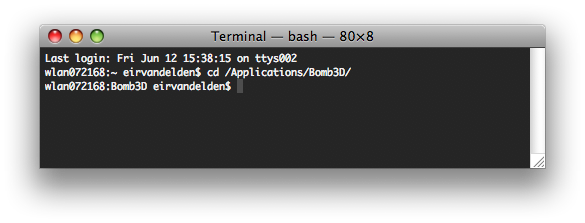
\includegraphics[width=14cm,height=5.5cm]{diagrams/directory}
          \caption{Changing to the installation directory} \label{fig:directory}
        \end{figure}
        
        Then run the command shown in Figure~\ref{fig:run_game}.
        
        \begin{figure}[!ht]
          \centering
          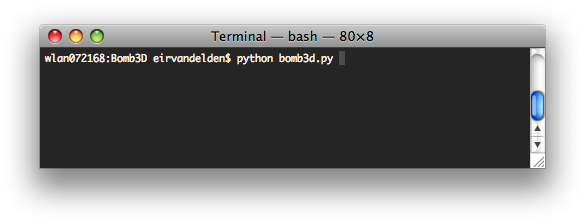
\includegraphics[width=14cm,height=5.5cm]{diagrams/run_game}
          \caption{Running Bomb3D} \label{fig:run_game}
        \end{figure}
        
    % section starting_the_game (end)

% chapter installation (end)

\chapter{Playing the Game} % (fold)
\label{cha:playing_the_game}
    
    \section{Joining a game}

    After starting Bomb3D, you can search for a game by pressing ``s''. Then choose a game of your liking by pressing the corresponding number key and start playing!
    
    
    \section{Starting a game} % (fold)
    \label{sec:starting_a_game}
        After starting Bomb3D, you can start a game by pressing ``c''. Fill in a new name if you like and then press ``d'' to start. Players can now join the game. After 15 seconds, the game is started. \footnote{Please note that Bomb3D can only play either in server mode or in client mode. To play with your friends, open Bomb3D twice (once to start server, once to connect to it). After the game has started, you can close the server. Note also that the game will not run if the creator is the only player.}.
        
    % section starting_a_game (end)
    
    \section{Let's Play!}

    Bomb3D is played using the mouse and keyboard.

    While in a game, the player can use the mouse to look around. There's a default assignment of mouse buttons and keys to actions.

    The default input configuration is as follows: The player moves around using the $W$, $A$, $S$ and $D$ keys. $W$ moves the avatar forward, $S$ moves him backward, and $A$/$D$ is used to move sideways. Bombs are dropped using the left mouse button. The numeric keys are used to activate the corresponding power-up.

    List with input keys:
     \begin{itemize}
        \item $W$: Move forward.
        \item $S$: Move backward.
        \item $A$: Step sideways (left).
        \item $D$: Step sideways (right).
        \item $1$: Activate power-up 1.
        \item $2$: Activate power-up 2.
        \item $3$: Activate power-up 3.
        \item $Mouse Movement$: Look around.
        \item $Left Mouse Button$: Drop Bomb.
     \end{itemize}
    
    \section{Power-ups}

    In bomb3D, you can find exciting and interesting power-ups to enhance your performance. Here's a list with all the available power-ups:

\begin{powerup}[Extra Bomb]
       Each player starts with one bomb in his arsenal, which means he can drop one bomb at one time, he can only drop a new bomb after the last bomb has exploded. When a player picks up the extra bomb power-up, the player gets an additional bomb he can place on the map. 
\end{powerup}

\begin{powerup}[Increase range]
        Bombs have a certain range, all players start with a bomb range of one. When a player picks up the range power-up, his or her bombs will increase in range.
\end{powerup}
% chapter playing_the_game (end)



\end{document}
